\section{Screening and the loss-function rate}\label{sec:10.2}

At a momentum transfer of \SI{2}{keV} the static dielectric function of silicon is about 2.9, and a potential that varies on that scale reaches the valence electrons weakened by $1/|\varepsilon|^2 \approx 0.12$. Yet the screened rate of a \SI{10}{MeV} particle with a heavy mediator is only 2.3 times smaller than the unscreened rate of \cref{sec:10.1}. The rate is an integral over all the momentum transfers and energies that kinematics allows, most of which lie where the medium screens little, and over a spectrum whose total weight screening cannot change. Two sum rules of the loss function bound it from above, with only the plasma frequency and the static dielectric function as input. The bound on the static step fails for a mediator that couples to electrons alone once the lattice is free to move, because the electrons that follow the nuclei add an acoustic peak.

\subsection{The loss-function rate}\label{sec:10.2-rate}

A mediator that couples to the electron number acts on one row of the master formula, the density $n_e(\vect{q})$, with $\mathfrak{D}_{ee} = |\tilde V(\vect{q})|^2 = \pi\sigmae\FDM(q)^2/\mu_{\chi e}^2$ (\cref{eq:1.4-Vsq}), and the spectrum \cref{eq:8.2-spectrum} needs only the structure factor $S_{ee}$. \Cref{sec:10.1} computed it for independent electrons. The exact structure factor follows from the fluctuation--dissipation theorem as $S = (2q^2/e^2)\,L/(1 - \ee^{-\beta\omega})$, with $L(\vect{q},\omega) = \Imag[-(\varepsilon^{-1})_{\vect{0}\vect{0}}(\vect{q},\omega)]$ the loss function of \cref{eq:4.4-SL}, and the exactness theorem \cref{eq:8.4-exact} says for which couplings this holds. For a dark photon, or any mediator that couples to the total charge $n_Z$, it holds at every $(\vect{q},\omega)$ with the loss function of the total dielectric matrix of electrons and nuclei. For a mediator that couples to electrons and not to nucleons it holds exactly only with the nuclei clamped. Above the phonon band the nuclei reach the electronic final states through the Migdal amplitudes alone, suppressed by powers of $\kappa_{\mathrm{BO}}$, and the loss function gives the electron-only rate to that accuracy (\cref{sec:8.4-exact}). An electron--hole pair in silicon costs at least \SI{1.17}{eV}, eighteen times the top of the phonon band, so for the electronic rate the two couplings share one formula. In silicon the Born charges vanish, and the ionic part of the total dielectric function at these energies is negligible.

Inserting $S$ into \cref{eq:8.2-spectrum}, with $e^2 = 4\pi\alpha$, gives $|\tilde V|^2 S = \sigmae\FDM^2q^2L/[2\alpha\mu_{\chi e}^2(1 - \ee^{-\beta\omega})]$ under the integrals~\cites[Eq.~(13)]{knapen2021dark}[Eq.~(1)]{hochberg2021determining}. For an isotropic target, or a crystal whose loss function is averaged over the directions of $\vect{q}$, the velocity integral and the angular integral act on the delta function alone and produce the measure $q\,\dd q\,\eta(\vmin)/4\pi^2$ of \cref{eq:A.8-eta}, with $\vmin = \omega/q + q/2\mchi$ from \cref{eq:1.3-vmin}. Collecting the factors,
\begin{keyresult}[Loss-function rate]
\begin{equation}
  \frac{\dd\mathcal{R}}{\dd\omega} = \frac{\rho_\chi\,\sigmae}{8\pi^2\alpha\,\rho_T\,\mchi\,\mu_{\chi e}^2}\int\dd q\;q^3\,\eta\bigl(\vmin(q,\omega)\bigr)\,\FDM(q)^2\,\frac{\bar L(q,\omega)}{1 - \ee^{-\beta\omega}} ,
  \label{eq:10.2-rate}
\end{equation}
with $\bar L$ the loss function averaged over the directions of $\vect{q}$. It is exact for a coupling to the total charge, and for a coupling to the electron density at clamped nuclei or above the phonon band to Migdal order.
\end{keyresult}
\noindent At the temperatures of a detector $\beta\Eg$ is of order $10^4$ or more, and the factor $1/(1 - \ee^{-\beta\omega})$ is one. All of the medium's physics is now in one measurable function. Screening is in it through the inverse of the dielectric matrix, and so are the local fields, because $L$ is a diagonal element of $\varepsilon^{-1}$ and not the inverse of a diagonal element of $\varepsilon$. For a momentum transfer beyond the first zone the element is the one at the reciprocal vector $\vect{G}_q$ of the unreduced $\vect{q} = \vect{q}_r + \vect{G}_q$, $L = \Imag[-(\varepsilon^{-1})_{\vect{G}_q\vect{G}_q}(\vect{q}_r,\omega)]$. A crystal has a loss function that depends on the direction of $\vect{q}$, and a rate at a fixed time keeps the full kernel of \cref{app:A.8} in place of $\eta/2q$. In a cubic crystal the first anisotropic term of $L$ has angular momentum four, and it is the source of the daily modulation of \cref{sec:11.7}.

The rate of \cref{sec:10.1} is the same formula with $L$ replaced by $\varepsilon_2$ of the independent-particle head: since $S^{\mathrm{IP}} = -2\Imag R^0_{\vect{0}\vect{0}}$ (\cref{sec:10.1}) and $\varepsilon_2 = -v_{\mathrm{C}}(q)\Imag R^0_{\vect{0}\vect{0}}$ (\cref{eq:4.6-R0}), $S^{\mathrm{IP}} = (2q^2/e^2)\,\varepsilon_2^{\mathrm{IP}}$. The prefactor is the one of \cref{eq:10.2-rate}, and \cref{eq:10.1-fcrys} is this relation rewritten as a form factor. Each many-body approximation of \cref{sec:4.6} is then a choice of what to put in place of $\bar L$. Independent particles put $\varepsilon_2^{\mathrm{IP}}$. The random-phase approximation without local fields puts $\varepsilon_2^{\mathrm{IP}}/|\varepsilon_{\vect{0}\vect{0}}|^2$, in which the head $\varepsilon_{\vect{0}\vect{0}} = 1 - v_{\mathrm{C}}(q)R^0_{\vect{0}\vect{0}}$ is inverted as a number. With local fields it is $\Imag[-(\varepsilon^{-1})_{\vect{0}\vect{0}}]$ with the full matrix of \cref{eq:4.6-rpaLF}. Exchange--correlation kernels and the electron--hole attraction change the proper response inside the same inverse (\cref{sec:4.6,sec:4.9}). The three rates differ only in the many-body approximation $\mathcal{X}$ of \cref{sec:8.5}, IP, RPA and RPA + LF, with every other entry of $\mathfrak{T}$ at its base value.

For a dark photon, \cref{eq:10.2-rate} uses the reference cross section with the vacuum mixing $\zeta$, and the loss function already contains the in-medium mixing. In scattering the dark photon mixes with the longitudinal photon of the medium, its propagator acquires the factor $1/\varepsilon(\vect{q},\omega)$, and that factor is the screening of the total-charge row (\cref{sec:8.4-mixing}). The vacuum mixing goes with the full response and the in-medium mixing with the proper one; multiplying \cref{eq:10.2-rate} by $\zeta_{\mathrm{eff}}^2/\zeta^2$ would count the screening twice.

The loss function is computed from Kohn--Sham states: the random-phase dielectric matrix with local fields is inverted at each $(\vect{q}_r,\omega)$, and the diagonal element is read off at $\vect{G}_q$ (\cref{app:E.6}). Two kinds of measurement test it: optical constants give $L$ at $q \to 0$, the curve of \cref{fig:4-siloss}, and electron energy-loss and inelastic x-ray scattering give it at finite $q$. The silicon tables used below are a published calculation of this kind~\cite{knapen2021dark}, distributed with the DarkELF code~\cite{knapen2022darkelf}. They use Kohn--Sham states with the gap fixed by a scissor shift, a $\vect{k}$ grid of $8^3$ and 70 bands, and give the dielectric matrix with and without local fields. They extend to $q = \SI{22.5}{keV}$ and $\omega = \SI{89}{eV}$. Kinematics keeps the rate inside them, since $\omega \le qv_{\mathrm{max}}$ is below \SI{60}{eV} for every momentum of the table. For a material without such tables, the Mermin oscillator method of \cref{sec:4.5} fits the measured optical loss function, gap and absorption peaks included, and carries each term to finite $q$ with its share of the $f$-sum. For silicon it agrees with the first-principles tables to within 10 percent in the rate above a two-electron threshold, and the uncertainty grows for masses whose rate lies near the gap~\cite[App.~C]{knapen2021dark}.

\begin{limitbox}[Loss-function rate][lim:10.2a]
For a coupling to the electron density or to the total charge, the spectrum per unit target mass is $\dd\mathcal{R}/\dd\omega = [\rho_\chi\sigmae/(8\pi^2\alpha\rho_T\mchi\mu_{\chi e}^2)]\int\dd q\,q^3\eta(\vmin)\FDM^2\,\Imag[-1/\varepsilon(q,\omega)]/(1 - \ee^{-\beta\omega})$~\cites[Eqs.~(6) and (13)]{knapen2021dark}[Eq.~(1)]{hochberg2021determining}.
\par\smallskip
{\centering
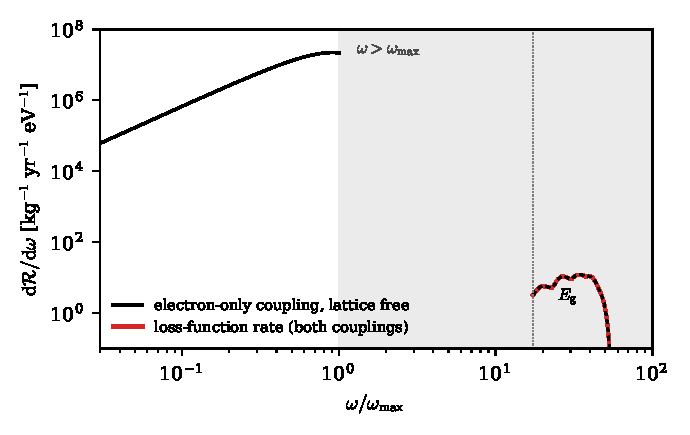
\includegraphics[width=0.82\linewidth]{figures/ch10/limit10_2a.pdf}
\captionof{figure}{Spectrum of silicon at $\mchi = \SI{1}{MeV}$, heavy mediator, $\sigmae = \SI{e-37}{cm^2}$, against $\omega/\omega_{\max}$, with $\omega_{\max} = \SI{64.1}{meV}$ the top of the phonon band. Red: the loss-function rate with the random-phase loss function with local fields; it is the whole rate of a dark photon, since the Born charges of silicon vanish. Black: an electron-only coupling with the lattice free to move, which adds the acoustic peak carried by the electrons that follow the nuclei. Model of the peak: isotropic linear longitudinal branch with $c_{\mathrm{LA}} = \SI{8.43}{km/s}$ up to $|\vect{q}| = 2\pi/a$, 14 electrons per atom following rigidly, no Debye--Waller factor, no Umklapp, transverse or multiphonon terms. Gray: $\omega > \omega_{\max}$, where the two couplings share the loss-function rate; dotted, the gap.}\label{fig:10-elf-limit}
\par}
\smallskip
Inside the phonon band an electron-only coupling excites acoustic phonons through the electrons that move with the nuclei, a peak that the loss function of the total charge does not have and that, in this model, carries more than $10^4$ times the electronic rate.
\end{limitbox}

\subsection{Screening corrections in silicon}\label{sec:10.2-corrections}

\Cref{fig:10-screening} shows the silicon rate in the three approximations. At \SI{10}{MeV} with a heavy mediator the spectrum peaks near \SI{5}{eV} in each of them, and only its height changes. Per kilogram-year at $\sigmae = \SI{e-37}{cm^2}$ the total above the gap is $1.36\times10^5$ events for independent particles, from the independent-particle head of these tables and not from the form-factor table of \cref{sec:10.1}, which gives $1.60\times10^5$ (\cref{sec:10.10-manybody} traces the difference), $8.6\times10^4$ in the random-phase approximation without local fields and $5.9\times10^4$ with them. The ratio of the unscreened rate to the screened one with local fields is 2.3 for a heavy mediator and 3.7 for a light one, and above about \SI{10}{MeV} it hardly depends on the mass. Below a few MeV it rises steeply, to 9 and 13 at \SI{1}{MeV}. At \SI{3}{MeV} it is 2.8 for a heavy mediator and 5.1 for a light one: random-phase screening lowers the independent-particle rate by \SI{52}{\percent}, and local fields lower what remains by a further \SI{26}{\percent}; for a light mediator the steps are \SI{76}{\percent} and \SI{18}{\percent}. The local fields alone lower the rate by a factor 1.46 for a heavy mediator and 1.27 for a light one at \SI{10}{MeV}, and by about 1.1 at \SI{1}{MeV}.

\begin{figure}[tbp]
  \centering
  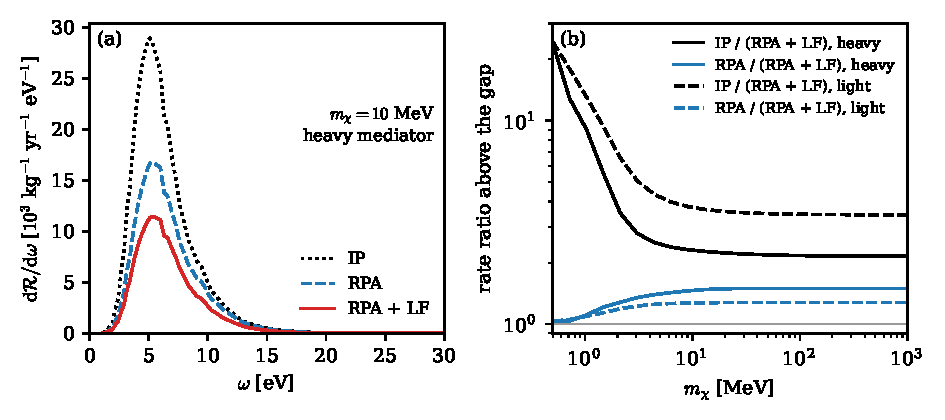
\includegraphics[width=\linewidth]{figures/ch10/fig10_2.pdf}
  \caption{Electron-recoil rate of silicon in three approximations, independent particles, RPA, and RPA with local fields, from the random-phase dielectric matrices of Knapen, Kozaczuk and Lin~\cite{knapen2021dark}, with and without local fields, with $\rho_\chi = \SI{0.3}{GeV.cm^{-3}}$, the standard halo of \cref{sec:1.2}, $\sigmae = \SI{e-37}{cm^2}$ and threshold \SI{1.11}{eV}, the step-model gap of pair creation that accompanies the tables (their scissor puts the gap at \SI{1.17}{eV}). IP: $\varepsilon_2$ of the independent-particle head of the same tables in place of $L$, the unscreened rate of \cref{sec:10.1} from a different tabulation; RPA: $\varepsilon_2/|\varepsilon_{\vect{0}\vect{0}}|^2$; RPA + LF: $\Imag[-(\varepsilon^{-1})_{\vect{0}\vect{0}}]$. The tabulated functions are averaged over the directions of $\vect{q}$ in bins of \SI{100}{eV} in $|\vect{q}|$, a choice of this figure, and end at $|\vect{q}| = \SI{22.5}{keV}$; momenta above \SI{15}{keV} already carry less than \SI{2}{\percent} of the rate at \SI{10}{MeV}. (a) Spectra at $\mchi = \SI{10}{MeV}$, heavy mediator. (b) Ratio of the rate above the gap to the rate with local fields, against $\mchi$; solid, heavy mediator, $\FDM = 1$; dashed, light mediator, $\FDM = (q_0/q)^2$.}
  \label{fig:10-screening}
\end{figure}

A pointwise screening factor would suggest a larger effect. The static values of the same tables give $\varepsilon(q,0) = 2.87$ at \SI{2}{keV} and 1.76 at $q_0 = \SI{3.73}{keV}$, so $1/\varepsilon^2$ is 0.12 and 0.32. At finite frequency the factor is stronger still: at $q_0$ the ratio $\varepsilon_2^{\mathrm{IP}}/L$ is 4.7 at \SI{3}{eV}, 5.2 at \SI{5}{eV} and 4.4 at \SI{10}{eV}. A pointwise factor leaves out where in $q$ the rate comes from, the $f$-sum rule, and the local fields, and these set the rate ratio of 2.3.

Consider first which momentum transfers carry the rate. With a heavy mediator, $q^3\eta(\vmin)$ weights large momentum transfers until the kinematic edge closes them, and at \SI{10}{MeV} half of the screened rate comes from $q > \SI{6.7}{keV}$ and \SI{29}{\percent} from $q > 2q_0$. There the valence electrons barely screen. At \SI{8}{keV} the static factor is 0.87, and the head screening, the ratio of the independent-particle rate to the random-phase rate without local fields at that momentum, is 1.18, against 13 at \SI{2}{keV} and 4.2 at $q_0$. A light mediator weights the small momenta, where screening is strong, and its ratio is correspondingly larger.

The $f$-sum rule is the second. Screening does not remove spectral weight, since $\int\dd\omega\,\omega L$ and $\int\dd\omega\,\omega\varepsilon_2$ are both $(\pi/2)\omega_p^2$ at every $\vect{q}$ (\cref{eq:4.4-fsumL,eq:4.4-fsumeps}); it moves the weight from the transition energies up toward the plasmon. At $q_0$ the peak of $\varepsilon_2^{\mathrm{IP}}$ lies at \SI{14}{eV} and that of $L$ at \SI{26}{eV}. Whether the moved weight is lost depends on the largest energy the dark matter can deposit, $\mchi v_{\mathrm{max}}^2/2$. At \SI{10}{MeV} this is \SI{35}{eV}, the moved weight stays mostly in reach, and the mean energy of the heavy-mediator spectrum rises only from 6.2 to \SI{6.6}{eV}. At \SI{1}{MeV} it is \SI{3.5}{eV}, the rate samples only the depleted low-energy side of $L$, and the ratio grows to 9. This is why the curves of \cref{fig:10-screening}b turn up at small mass.

The local fields are the third, and at the momenta that carry the heavy-mediator rate they are larger than the head screening. Per unit momentum transfer, the rate without local fields exceeds the rate with them by 1.17 at $q_0$, 1.67 at \SI{8}{keV} and 1.83 at \SI{10}{keV}, two to three times the shortest reciprocal-lattice vector $|\vect{G}_{111}| = \SI{3.95}{keV}$. The reason is the crystal potential. A density wave at $\vect{q} = \vect{q}_r + \vect{G}_q$ induces, through the Bloch states, charge at every $\vect{q}_r + \vect{G}$, including the long-wavelength component at $\vect{q}_r$ itself, whose Coulomb field $v_{\mathrm{C}}(|\vect{q}_r|)$ is large and acts back. The head-only random-phase approximation keeps only the diagonal element and misses this field; the inverse of the full matrix contains it. An all-electron calculation with local fields finds the same suppression of the structure factor above about $3\alpha m_e$, and a reduction of the projected reach by 20 to \SI{50}{\percent} for masses above a few MeV~\cite{dreyer2026all}. The size is not settled. At \SI{10}{keV} the energies below \SI{89}{eV} hold only \SI{17}{\percent} of the $f$-sum, the rest lying near the free recoil at $q^2/2m_e = \SI{98}{eV}$ and above. The rate samples the far low-energy tail of the spectrum, and the tail is sensitive to the band count and the pseudopotential. The spread between published calculations at these momenta is part of the many-body uncertainty of the rate (\cref{sec:8.8}). A local empirical pseudopotential that shares no input with the tables but the crystal structure shows the same suppression (\cref{fig:10-fcrys-limit,sec:10.10-manybody}). In that model at \SI{5}{eV} the kinematic edge lies at $0.525\,q_0$; just above it, at $q = 0.55\,q_0$, screening cuts the response to 0.05 of the independent-particle value, and at $q_0$ to 0.22. Integrated over $q$, the screened rate at \SI{5}{eV} is 0.47 of the independent-particle one.

\begin{figure}[tbp]
  \centering
  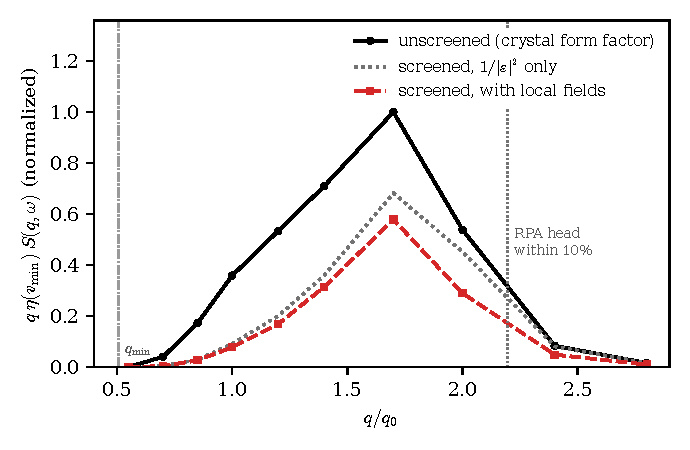
\includegraphics[width=0.85\linewidth]{figures/ch10/limit10_1a.pdf}
  \caption{Unscreened rate against screened rates in silicon at $\omega = \SI{5}{eV}$, for $\mchi = \SI{10}{MeV}$ and a heavy mediator: the rate weight $q\,\eta(\vmin)\,S(q,\omega)$ of \cref{eq:10.1-rateiso} against $q$, normalized to the maximum of the unscreened curve. All three curves come from one model, the local empirical pseudopotential of \cref{we:8-lf-nuisance} (model gap \SI{0.82}{eV}), with $\vect{q}$ along the direction $(5,3,1)$, chosen so that no $\vect{q} + \vect{G}$ comes close to zero, and spectra averaged over 4.5 to \SI{5.5}{eV}. Solid: independent particles. Dotted: random-phase screening by the macroscopic $1/|\varepsilon|^2$ alone, the leading correction. Dashed: random-phase screening with local fields over the 51 shortest reciprocal-lattice vectors, the fuller result. Dash-dotted: the smallest $q$ the halo reaches at \SI{5}{eV}. Dotted vertical: above $2.2\,q_0 = \SI{8.2}{keV}$, with $q_0 = \alpha m_e$, the macroscopic screening changes the rate by less than 10 percent. The model has no momentum components above $2.8\,q_0$, where the plot ends. Nothing is shaded. No $q$ in the plotted range brings the fuller result within 10 percent of the unscreened one.}
  \label{fig:10-fcrys-limit}
\end{figure}

The further corrections, an exchange--correlation kernel and the electron--hole attraction, change the picture mainly near the gap. An adiabatic local kernel changes the loss function by a few percent at energies of several eV, since it cannot bind an electron to a hole (\cref{sec:4.6}). The electron--hole attraction raises the spectrum within about an eV of the gap and adds bound excitons below it (\cref{sec:4.9}); \cref{sec:10.5} computes its effect on the rate. The optical limit of the tables shows what is missing at small $q$: $\varepsilon(0,0)$ is 10.2 without local fields and 9.1 with them, against the measured 11.7, the same trend as \cref{we:4-siepsinf}. A rate dominated by the region just above the gap, as for masses of a few MeV, inherits that uncertainty, and a heavier one is less sensitive to it.

\subsection{Sum-rule bounds on the rate}\label{sec:10.2-bounds}

Silicon has 28 electrons per cell, and the $f$-sum rule fixes $\int_0^\infty\dd\omega\,\omega L$ at $(\pi/2)\omega_p^2$ with $\omega_p = \SI{31.1}{eV}$ for all of them (\cref{sec:4.3}), whatever the bands, the screening or the many-body approximation. The inverse moment is fixed by the static dielectric function alone. These two integrals bound the rate of \cref{eq:10.2-rate} from above, for any material, with no calculation of the spectrum~\cites{lasenby2022dark}{barker2026first}. Define the moments of the loss function at fixed $\vect{q}$,
\begin{equation}
  K_n(\vect{q}) = \int_0^\infty\dd\omega\;\omega^n L(\vect{q},\omega) , \qquad
  K_1 = \frac{\pi}{2}\,\omega_p^2 , \qquad K_{-1} = \frac{\pi}{2}\bigl[1 - \varepsilon^{-1}(\vect{q},0)\bigr] ,
  \label{eq:10.2-moments}
\end{equation}
where $K_1$ is \cref{eq:4.4-fsumL} and $K_{-1}$ is the Kramers--Kronig relation \cref{eq:C.5-screening} at zero frequency, at which $\varepsilon^{-1}$ is real. At $\vect{q} \to 0$ in an insulator the second is the inverse moment \cref{eq:4.4-inverse}; at finite $q$ it is the static step $1 - \varepsilon^{-1}(\vect{q},0)$, which falls from 0.87 at \SI{0.5}{keV} to 0.43 at $q_0$ and 0.28 at \SI{5}{keV} in the silicon tables.

The intermediate moments follow by Hölder's inequality. For $-1 \le n \le 1$ write $\omega^nL = (\omega L)^{(1+n)/2}(L/\omega)^{(1-n)/2}$, a product of two nonnegative functions, and apply $\int fg \le (\int f^r)^{1/r}(\int g^s)^{1/s}$ with $r = 2/(1+n)$ and $s = 2/(1-n)$, so that $1/r + 1/s = 1$. Then $K_n \le K_1^{(1+n)/2}K_{-1}^{(1-n)/2}$, or
\begin{equation}
  K_n(\vect{q}) \le \frac{\pi}{2}\,\omega_p^{n+1}\bigl[1 - \varepsilon^{-1}(\vect{q},0)\bigr]^{(1-n)/2} , \qquad -1 \le n \le 1 ,
  \label{eq:10.2-Kn}
\end{equation}
which is Ref.~\cite[Eq.~(8)]{barker2026first}; the end points are the two sum rules themselves, and $n = 0$ is the Cauchy--Schwarz inequality. In the rate, the halo factor $\eta(\vmin)$ is the only other function of $\omega$. At $T = 0$ and for energies above a threshold $\omega_{\mathrm{th}}$, write $\eta \le \omega^n\eta_n^{\max}(q)$ with $\eta_n^{\max}(q) = \max_{\omega \ge \omega_{\mathrm{th}}}\omega^{-n}\eta(\vmin(q,\omega))$, extend the energy integral down to zero, which only adds positive terms since $L \ge 0$ for $\omega > 0$, and use \cref{eq:10.2-Kn}:
\begin{equation}
  \mathcal{R} \le \frac{\rho_\chi\,\sigmae\,\omega_p^{n+1}}{16\pi\alpha\,\rho_T\,\mchi\,\mu_{\chi e}^2}\int\dd q\;q^3\,\FDM(q)^2\,\eta_n^{\max}(q)\,\bigl[1 - \varepsilon^{-1}(q,0)\bigr]^{(1-n)/2} ,
  \label{eq:10.2-bound}
\end{equation}
Ref.~\cite[Eq.~(9)]{barker2026first}. The case $n = -1$ uses the static step alone and is the bound of Lasenby and Prabhu~\cite[Eqs.~(8) and (9)]{lasenby2022dark}. Every $n$ gives a valid bound, and the best one at a given mass is the smallest.

The useful form of the inverse moment needs $0 \le 1 - \varepsilon^{-1}(q,0) \le 1$. The lower limit is positivity: $1 - \varepsilon^{-1} = -v_{\mathrm{C}}R(\vect{q},0)$, and a static density response is negative by its Lehmann form (\cref{eq:4.2-positivity}). The upper limit, $\varepsilon^{-1}(\vect{q},0) \ge 0$, is not guaranteed in general, although we can show that it holds in the random-phase approximation with local fields for any insulator. The static independent-particle matrix $R^0_{\vect{G}\vect{G}'}(\vect{q},0)$ is Hermitian and negative semidefinite, each pair of states adding a positive rank-one matrix divided by minus its excitation energy, and so is $X = v^{1/2}R^0v^{1/2}$, with $v$ the diagonal matrix of $v_{\mathrm{C}}(|\vect{q}+\vect{G}|)$. The random-phase response gives $v^{1/2}Rv^{1/2} = X(1 - X)^{-1}$, whose eigenvalues $\lambda/(1 - \lambda)$, with $\lambda \le 0$, lie in $(-1, 0]$. A diagonal element of a Hermitian matrix lies between its smallest and largest eigenvalue, so $(\varepsilon^{-1})_{\vect{G}\vect{G}} = 1 + v_{\mathrm{C}}R_{\vect{G}\vect{G}}$ lies in $(0, 1]$ at every $\vect{q}$, local fields included. Beyond the random-phase approximation the same argument goes through with $R^0$ replaced by the proper response $\tilde R = (1 - R^0f_{\mathrm{xc}})^{-1}R^0$ of \cref{eq:4.6-tddft}, provided $\tilde R$ stays negative definite, that is $(-R^0)^{-1} + f_{\mathrm{xc}} > 0$. At long wavelength this is the positive inverse compressibility of \cref{eq:4.6-compress}, which the electron gas loses only near $r_s \approx 5.25$~\cite{giuliani2005quantum}, far from the $r_s \approx 2$ of the silicon valence electrons. For an arbitrary material a negative static dielectric function at finite $q$ is not excluded~\cite{dolgov1981admissible}, and the conservative replacement $1 - \varepsilon^{-1} \to 1$ that makes \cref{eq:10.2-bound} material-independent is an assumption there, not a theorem.

The bound applies to the total charge as well. For a dark photon the loss function and the static step are those of the total dielectric matrix of \cref{sec:8.4}, and the $f$-sum includes the nuclei, $\omega_p^2 + \sum_\kappa Z_\kappa^2e^2\nd_\kappa/M_\kappa$. In silicon the nuclear share is $2.73\times10^{-4}$ (\cref{sec:4.3}) and the Born charges vanish, so the numbers are those of the electrons. The inverse moment also gives a check on calculations. The unscreened $\varepsilon_2^{\mathrm{IP}}$ has $(2/\pi)\int\dd\omega\,\varepsilon_2/\omega = \varepsilon_{\vect{0}\vect{0}}(\vect{q},0) - 1$, by the Kramers--Kronig relation for $\varepsilon - 1$ (\cref{eq:C.5-KKeps}), and this exceeds the bound $1 - 1/\varepsilon_{\vect{0}\vect{0}}$ on the screened $L$ by the factor $\varepsilon_{\vect{0}\vect{0}}(\vect{q},0)$, which is 6.3 at \SI{1}{keV} in silicon.

\begin{workedexample}{The $f$-sum bound on the silicon rate at \SI{1}{MeV}}\label{we:10-fsum}
Take $\mchi = \SI{1}{MeV}$, a heavy mediator, $\sigmae = \SI{e-37}{cm^2}$, $\rho_\chi = \SI{0.3}{GeV.cm^{-3}}$ and the threshold $\omega_{\mathrm{th}} = \SI{1.11}{eV}$ of a charge detector, the step-model gap that accompanies the tables. Pairs are kinematically open for $\omega_{\mathrm{th}}/v_{\mathrm{max}} = \SI{0.42}{keV} \le q \le 2\mchi v_{\mathrm{max}} = \SI{5.30}{keV}$ and $\omega \le \mchi v_{\mathrm{max}}^2/2 = \SI{3.51}{eV}$. The screened rate of \cref{eq:10.2-rate} with local fields is 16.7 events per kilogram-year (18.5 without local fields, 157 for independent particles).

For $n = 1$, $\eta(\vmin)/\omega$ decreases with $\omega$ at fixed $q$, since $\vmin$ grows with $\omega$, so its maximum is at the threshold, $\eta_1^{\max}(q) = \eta(\vmin(q,\omega_{\mathrm{th}}))/\omega_{\mathrm{th}}$. The bound \cref{eq:10.2-bound} then needs only $\omega_p$. With all 14 electrons per atom, $\omega_p = \SI{31.1}{eV}$, it gives $7.3\times10^7$ events per kilogram-year, $4\times10^6$ times the computed rate. The valence plasma frequency, $\omega_p^{\mathrm{val}} = \SI{16.6}{eV}$, would give $2.1\times10^7$, but it is not a bound, since the core electrons hold the rest of the $f$-sum and the inequality runs over the whole spectrum. The $n = 0$ bound with the static step of the tables gives $2.0\times10^6$, and $n = -1$ gives $5.5\times10^4$, 3300 times the computed rate; with the step replaced by one it is $9.3\times10^4$. The tables contain only the valence electrons, whose step is slightly smaller than the all-electron one, so the $n = -1$ figure is a little low as a bound.

The bounds are far above the rate because they place all of the weight of $L$ at the most favorable energy, while silicon puts it where a \SI{1}{MeV} particle cannot go. The $f$-sum weight is near the plasmon, around \SI{17}{eV} at small $q$, and in the cores at hundreds of eV; the window ends at \SI{3.5}{eV}, where the gap and the screening keep $L$ small. The inverse moment weights low energies and comes closest. At \SI{10}{MeV}, with a window reaching \SI{35}{eV}, the $n = -1$ bound is 16 times the computed rate and the $f$-sum bound $8.5\times10^5$ times, both evaluated, like the rate, for $q \le \SI{22.5}{keV}$, which is valid because the bound holds at each $q$. A sum-rule bound comes close to the rate only for a material whose loss function concentrates its weight near the kinematic edge, a plasmon at a few eV, which is what the electron gas of \cref{sec:10.3} and the low-dimensional plasmons of \cref{sec:16.2} provide.
\end{workedexample}

\subsection{Static step of a relaxing lattice}\label{sec:10.2-lattice}

For a mediator that couples to electrons alone, the exact relation is $S_{ee} = (2q^2/e^2)L_e/(1 - \ee^{-\beta\omega})$ with the electron-channel function $\varepsilon_e^{-1} = 1 + v_{\mathrm{C}}R_{ee}$ (\cref{app:A.7}), and both sum rules hold for $L_e$. The $f$-sum is unchanged: the double commutator of $n_e$ with the Hamiltonian involves only the kinetic energy of the electrons (\cref{sec:4.3}), so $\int\dd\omega\,\omega L_e = (\pi/2)\omega_p^2$ with the nuclei moving, and the acoustic peak of the electron-following sector takes the share $Z_\kappa m_e/M_\kappa = 2.73\times10^{-4}$ of it in silicon (\cref{eq:8.6-fsum-e}). The static step is a different matter. With the nuclei free to move, an electron-only probe at small $q$ compresses neutral matter: the electrons it displaces drag their nuclei along, and the crystal responds as an elastic medium.

The size follows from the acoustic peak. At small $q$ a longitudinal acoustic phonon moves each cell rigidly by $\vect{U}_{\vect{R}}$, and the electrons that follow the nuclei, all $\nd_e\Omega = 28$ per cell in silicon since the Born charges vanish, give the density row the term $-\ii\,\nd_e\Omega\sum_{\vect{R}}\ee^{-\ii\vect{q}\cdot\vect{R}}\,\vect{q}\cdot\vect{U}_{\vect{R}}$ (\cref{sec:8.4-exact}). One phonon of wavevector $\vect{q}$ displaces each cell by $(2M_{\mathrm{cell}}N\omega_{\vect{q}})^{-1/2}$ along its polarization, with $N$ cells in the volume $\Vol = N\Omega$. The squared matrix element is then $N(\nd_e\Omega)^2q^2/(2M_{\mathrm{cell}}\omega_{\vect{q}})$, and
\begin{equation*}
  S_{ee}^{\mathrm{ac}}(\vect{q},\omega) = \frac{\pi\nd_e^2\Omega\,q^2}{M_{\mathrm{cell}}\,\omega_{\vect{q}}}\,\delta(\omega - \omega_{\vect{q}}) , \qquad \omega_{\vect{q}} = c_{\mathrm{LA}}q ,
\end{equation*}
at $T = 0$, with $c_{\mathrm{LA}}$ the longitudinal sound speed, the $c_\nu$ of \cref{eq:5.2-sound} for the longitudinal branch. Its first moment, $\int\dd\omega\,\omega S/2\pi = \nd_e^2\Omega q^2/2M_{\mathrm{cell}}$, is $\nd_e\Omega\,m_e/M_{\mathrm{cell}}$ times the electronic $f$-sum $\nd_eq^2/2m_e$, the share quoted above. Its inverse moment is not small. With $L_e = (e^2/2q^2)(1 - \ee^{-\beta\omega})S_{ee}$, the peak adds $(2/\pi)\int\dd\omega\,L_e^{\mathrm{ac}}/\omega = e^2\nd_e^2\Omega/(M_{\mathrm{cell}}\,\omega_{\vect{q}}^2)$ to the static step, and
\begin{keyresult}[Static step of a relaxing lattice]
\begin{equation}
  1 - \varepsilon_e^{-1}(\vect{q},0) = \bigl[1 - \varepsilon_{\mathrm{cl}}^{-1}(\vect{q})\bigr] + \mathcal{G}_{\mathrm{rel}}(\vect{q}) , \qquad
  \mathcal{G}_{\mathrm{rel}}(\vect{q}) \to \frac{\varOmega_{P,e}^2}{(c_{\mathrm{LA}}q)^2} , \quad \varOmega_{P,e}^2 = \frac{e^2\nd_e^2}{\rho_T} ,
  \label{eq:10.2-relaxed}
\end{equation}
as $q \to 0$, with $\varepsilon_{\mathrm{cl}}$ the dielectric function at clamped nuclei, $\nd_e$ the density of all the electrons and $\rho_T = M_{\mathrm{cell}}/\Omega$. The lattice term grows as $(c_{\mathrm{LA}}q)^{-2}$ in every solid, polar or not. Its general form, a sum over branches with the electron-following charge $Z^{(e)}_\kappa(\vect{q})$ of each atom, is \cref{eq:E.16-step}.
\end{keyresult}
\noindent For silicon, $\nd_e = \SI{7.00e23}{cm^{-3}}$ and $\rho_T = \SI{2.33}{g.cm^{-3}}$ give $\varOmega_{P,e} = \SI{0.51}{eV}$, and with $c_{\mathrm{LA}} = \SI{8.43}{km/s}$ along $[100]$ (\cref{app:C.18}) the lattice term equals one at $q = \SI{18}{keV}$, far beyond the zone boundary. The limiting form is derived only as $q \to 0$. At finite $q$ the dispersion bends over and the electron-following charge falls below 14 per atom, at relative order $(qa)^2$ and in opposite directions; at \SI{1}{keV} the limiting form gives $3\times10^2$, and the true value there is only estimated to exceed $10^2$ (\cref{app:E.16}). Either way the step exceeds one by orders of magnitude throughout the zone, and the bound \cref{eq:10.2-bound} with $n = -1$, and with every $n < 1$ through the power $(1 - n)/2$, fails for an electron-only coupling once the lattice relaxes. Lasenby and Prabhu noted that phonon rates of electrophilic mediators exceed the sum-rule bounds of charge couplings~\cite[Sect.~VII]{lasenby2022dark}; \cref{eq:10.2-relaxed} gives the term responsible. It is the acoustic peak of $S_{ee}$ that the exactness theorem of \cref{sec:8.4} attributed to the electrons that follow the nuclei. Its amplitude is the coefficient of $\ii\vect{q}\cdot\vect{U}$ in the density row, the coupling per unit volume $c_1^{(e)}\nd_e$ of the electrons that move with the cells; for the charge this coefficient cancels between electrons and nuclei, and the peak is absent.

The clamped bound holds in every many-body approximation, with the proviso on $\tilde R$ above; the lattice term is harmonic and adiabatic, with one phonon in the final state. For the electron-only coupling the $f$-sum bound and a restricted static-step bound survive. The $f$-sum bound holds as it stands. And for a threshold above the phonon band the electron-following sector contributes nothing to $\int_{\omega_{\mathrm{th}}}^\infty\dd\omega\,L_e/\omega$ except through Migdal amplitudes, so the clamped step bounds that integral up to corrections in powers of $\kappa_{\mathrm{BO}}$ (\cref{sec:8.6}). A detector with an electronic threshold can use the clamped bound for either coupling; a calorimeter with a threshold in the phonon band cannot use it for an electrophilic mediator.

\begin{limitbox}[Sum-rule bounds on the loss function][lim:10.2b]
For any target in its ground state, $\int_0^\infty\dd\omega\,\omega L = (\pi/2)\omega_p^2$ and $\int_0^\infty\dd\omega\,L/\omega = (\pi/2)[1 - \varepsilon^{-1}(q,0)] \le \pi/2$, and with $\eta \le \omega^n\eta_n^{\max}$ they bound the rate as in \cref{eq:10.2-bound}~\cites[Eqs.~(1), (8) and (9)]{lasenby2022dark}[Eqs.~(1), (2), (8) and (9)]{barker2026first}.
\par\smallskip
{\centering
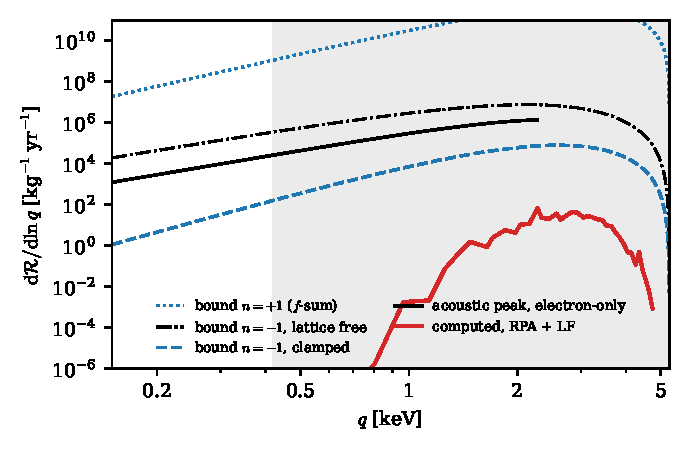
\includegraphics[width=0.82\linewidth]{figures/ch10/limit10_2b.pdf}
\captionof{figure}{Rate per unit $\ln q$ in silicon at $\mchi = \SI{1}{MeV}$, heavy mediator, $\sigmae = \SI{e-37}{cm^2}$, threshold \SI{1}{meV}, against the bounds of \cref{eq:10.2-bound}. Red: the computed electronic rate (random-phase loss function with local fields). Dashed: the clamped bound with $n = -1$ and the static step of the same tables; dotted: the $f$-sum bound, $n = 1$, $\omega_p = \SI{31.1}{eV}$. Black: the acoustic peak of an electron-only coupling, in the model of \cref{fig:10-elf-limit}; dash-dotted: the $n = -1$ bound with the lattice term \cref{eq:10.2-relaxed} added, in its limiting form $\varOmega_{P,e}^2/(c_{\mathrm{LA}}q)^2$ at every $q$ shown. Gray: momenta at which electron--hole pairs are open, $q \ge \Eg/v_{\mathrm{max}}$; there the clamped bound holds for both couplings when the threshold lies above the phonon band. The acoustic peak exceeds the clamped bound by 120 at \SI{0.5}{keV}, 42 at \SI{1}{keV} and 21 at \SI{2}{keV}.}\label{fig:10-sumrule-limit}
\par}
\smallskip
For an electron-only coupling with the lattice free to move, the static step grows as $(c_{\mathrm{LA}}q)^{-2}$ and exceeds one throughout the zone, and only the $f$-sum bound survives.
\end{limitbox}
